% SPDX-FileCopyrightText: 2024 Lukas Zirpel <thesis+lukas@zirpel.de>
% SPDX-License-Identifier: GPL-3.0-only

\chapter{Results}
\label{chap:results}
\todo{beschreiben, was man sieht, Messungen irgendwie anordnen, innerhalb Sektion mit anderem vergleichen, z.B. MTU. zuerst nach Protokollen, dann Parameter}

In this section, we describe the results obtained by performing our
experiments.


\section{RQ1: How much packet size overhead does each protocol add?}
While we aimed to quantify the precise packet size overhead introduced by each protocol, our experimental setup did not allow for direct measurement of this metric.
However, it is important to note that the packet size overheads of many protocols are generally constant.
This overhead is due to the protocol's header, which is added to the data payload.
\todo[inline]{break down overhead of WireGuard and ICMPTX}

\section{RQ2: How much does the MTU decrease by using each protocol?}
For protocols that do not support fragmentation by themselves, the MTU decrease is directly related to the protocol's overhead.

\section{RQ3: How much additional latency does each protocol add?}
cannot be measured with our measurement setup

\section{RQ4: Do any protocols introduce additional packet loss?}
cannot be measured with our measurement setup

\section{RQ5: How much processing power and RAM does each protocol consume/require?}
did not measure

for userspace tunnel programs, can be measured using systemctl status

Not sure how to measure RAM usage of WireGuard

WireGuard used approximately \% of one CPU core

determined by looking at the output ...


graphen beschreiben (Welche Achsen gibt es, etc.)
was sieht man?
warum sieht man das was man sieht?


graphs:
latency
packet counts
throughput

single or multi

single: axes:

for looking at a specific measurement in detail:

gives an overview of how consistent the measurement is

latency: box plot for every bucket: time, latency

packet counts: line with dot every bucket: time, counts

throughput: line with dot every bucket: time, throughput


to be able to see the influence of a parameter, multiple measurements in one graph:

\begin{figure}[tbh]
	\centering
	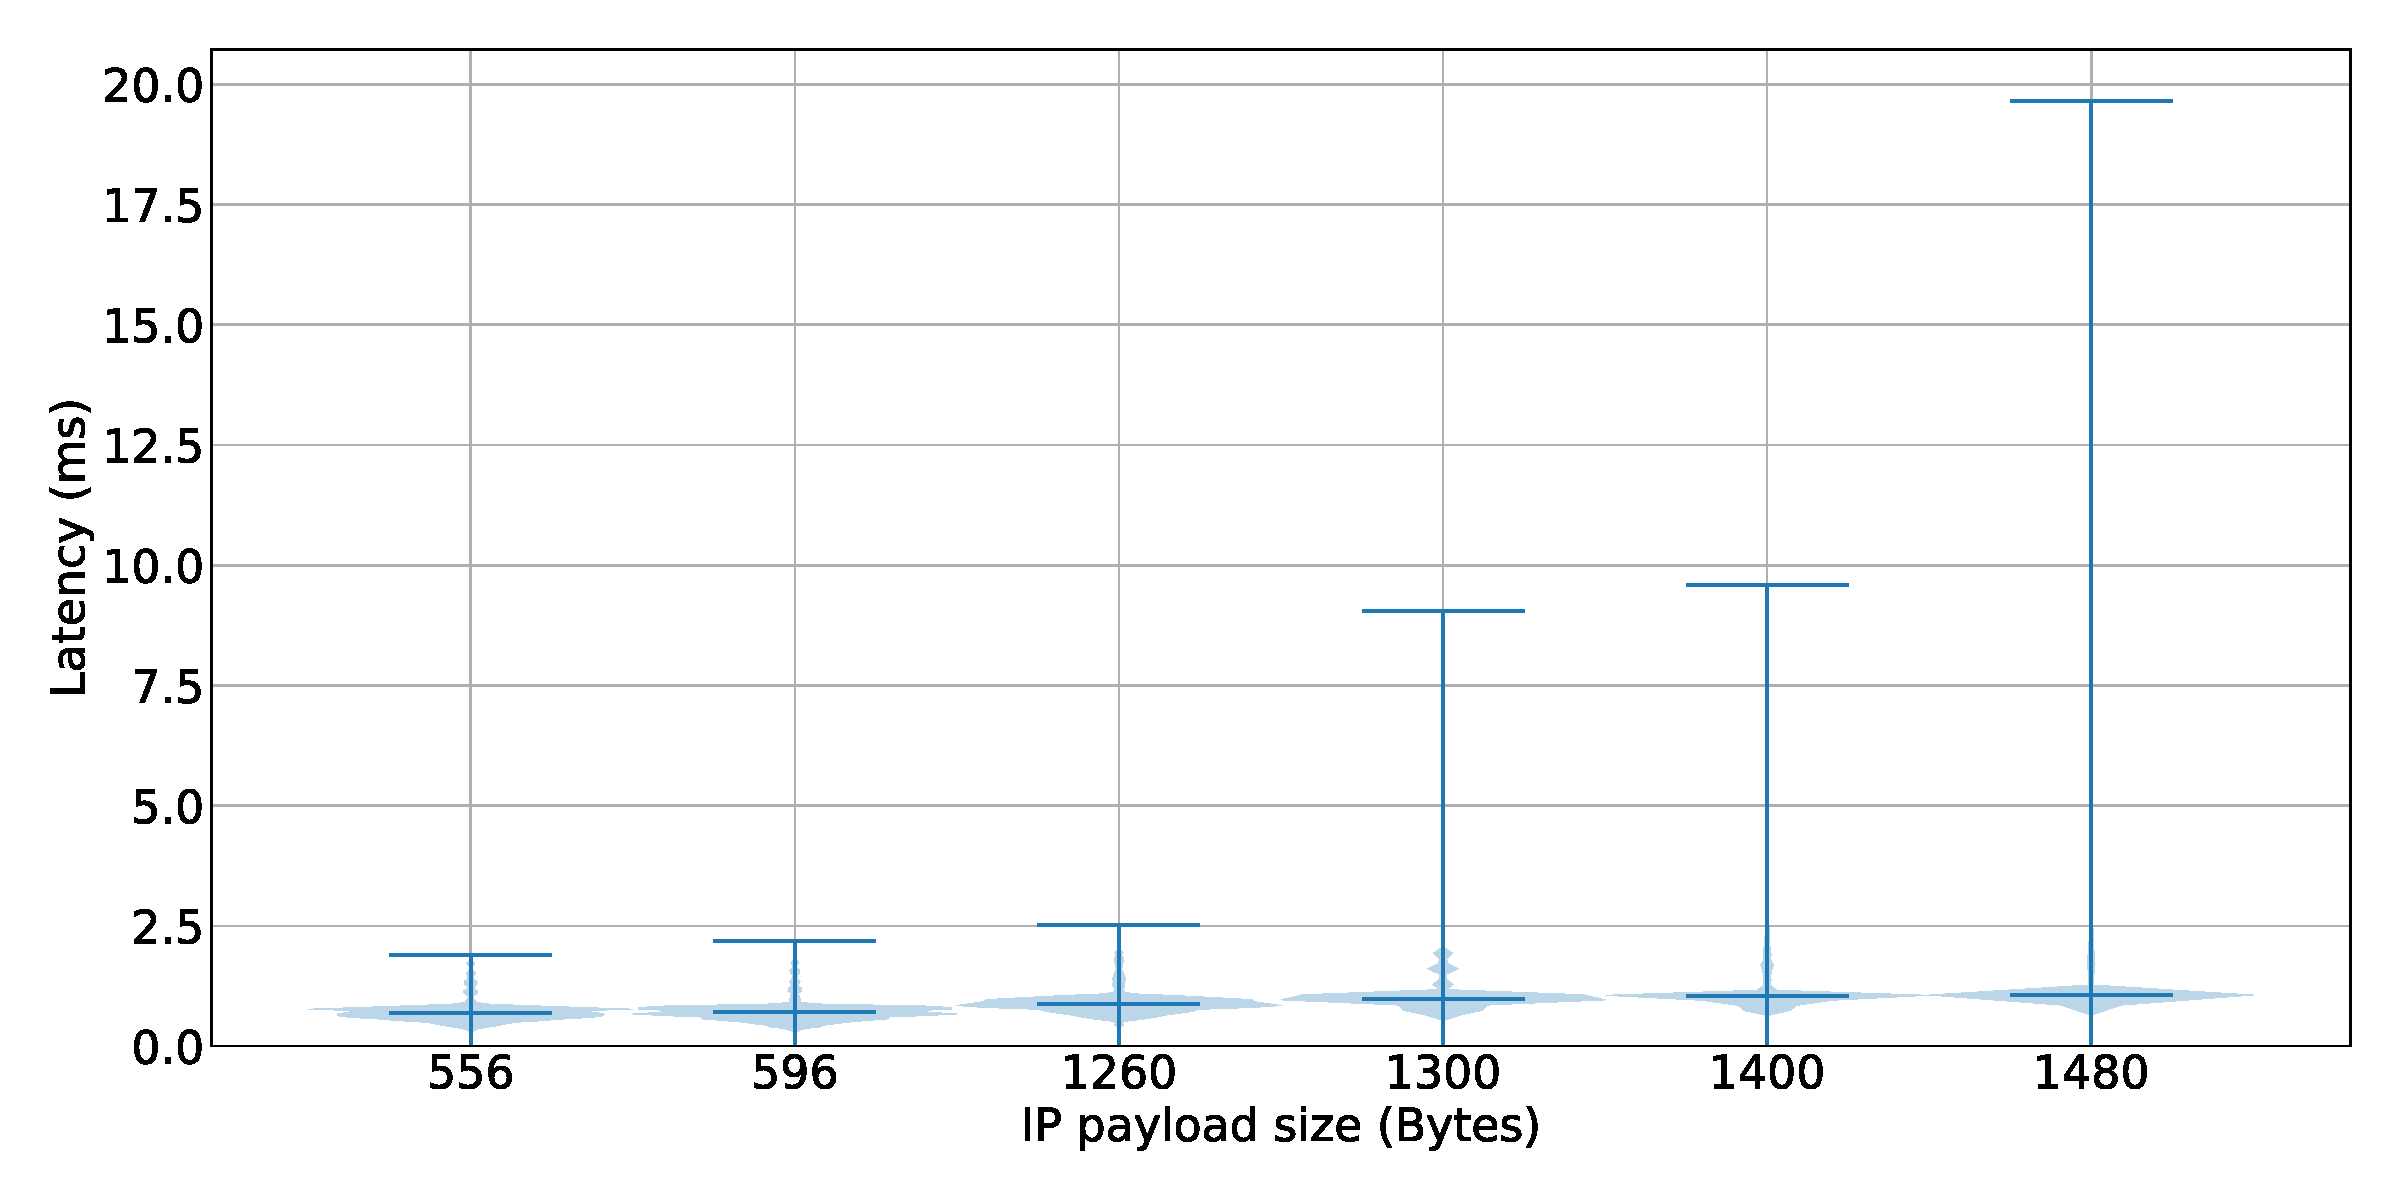
\includegraphics[draft=false,width=0.9\textwidth]{figures/Graphs/graph-1-mtu/latencies.pdf}
	\caption{Latencies for varying payload sizes}\label{fix:graph-1-mtu-latencies}
\end{figure}
\begin{figure}[tbh]
	\centering
	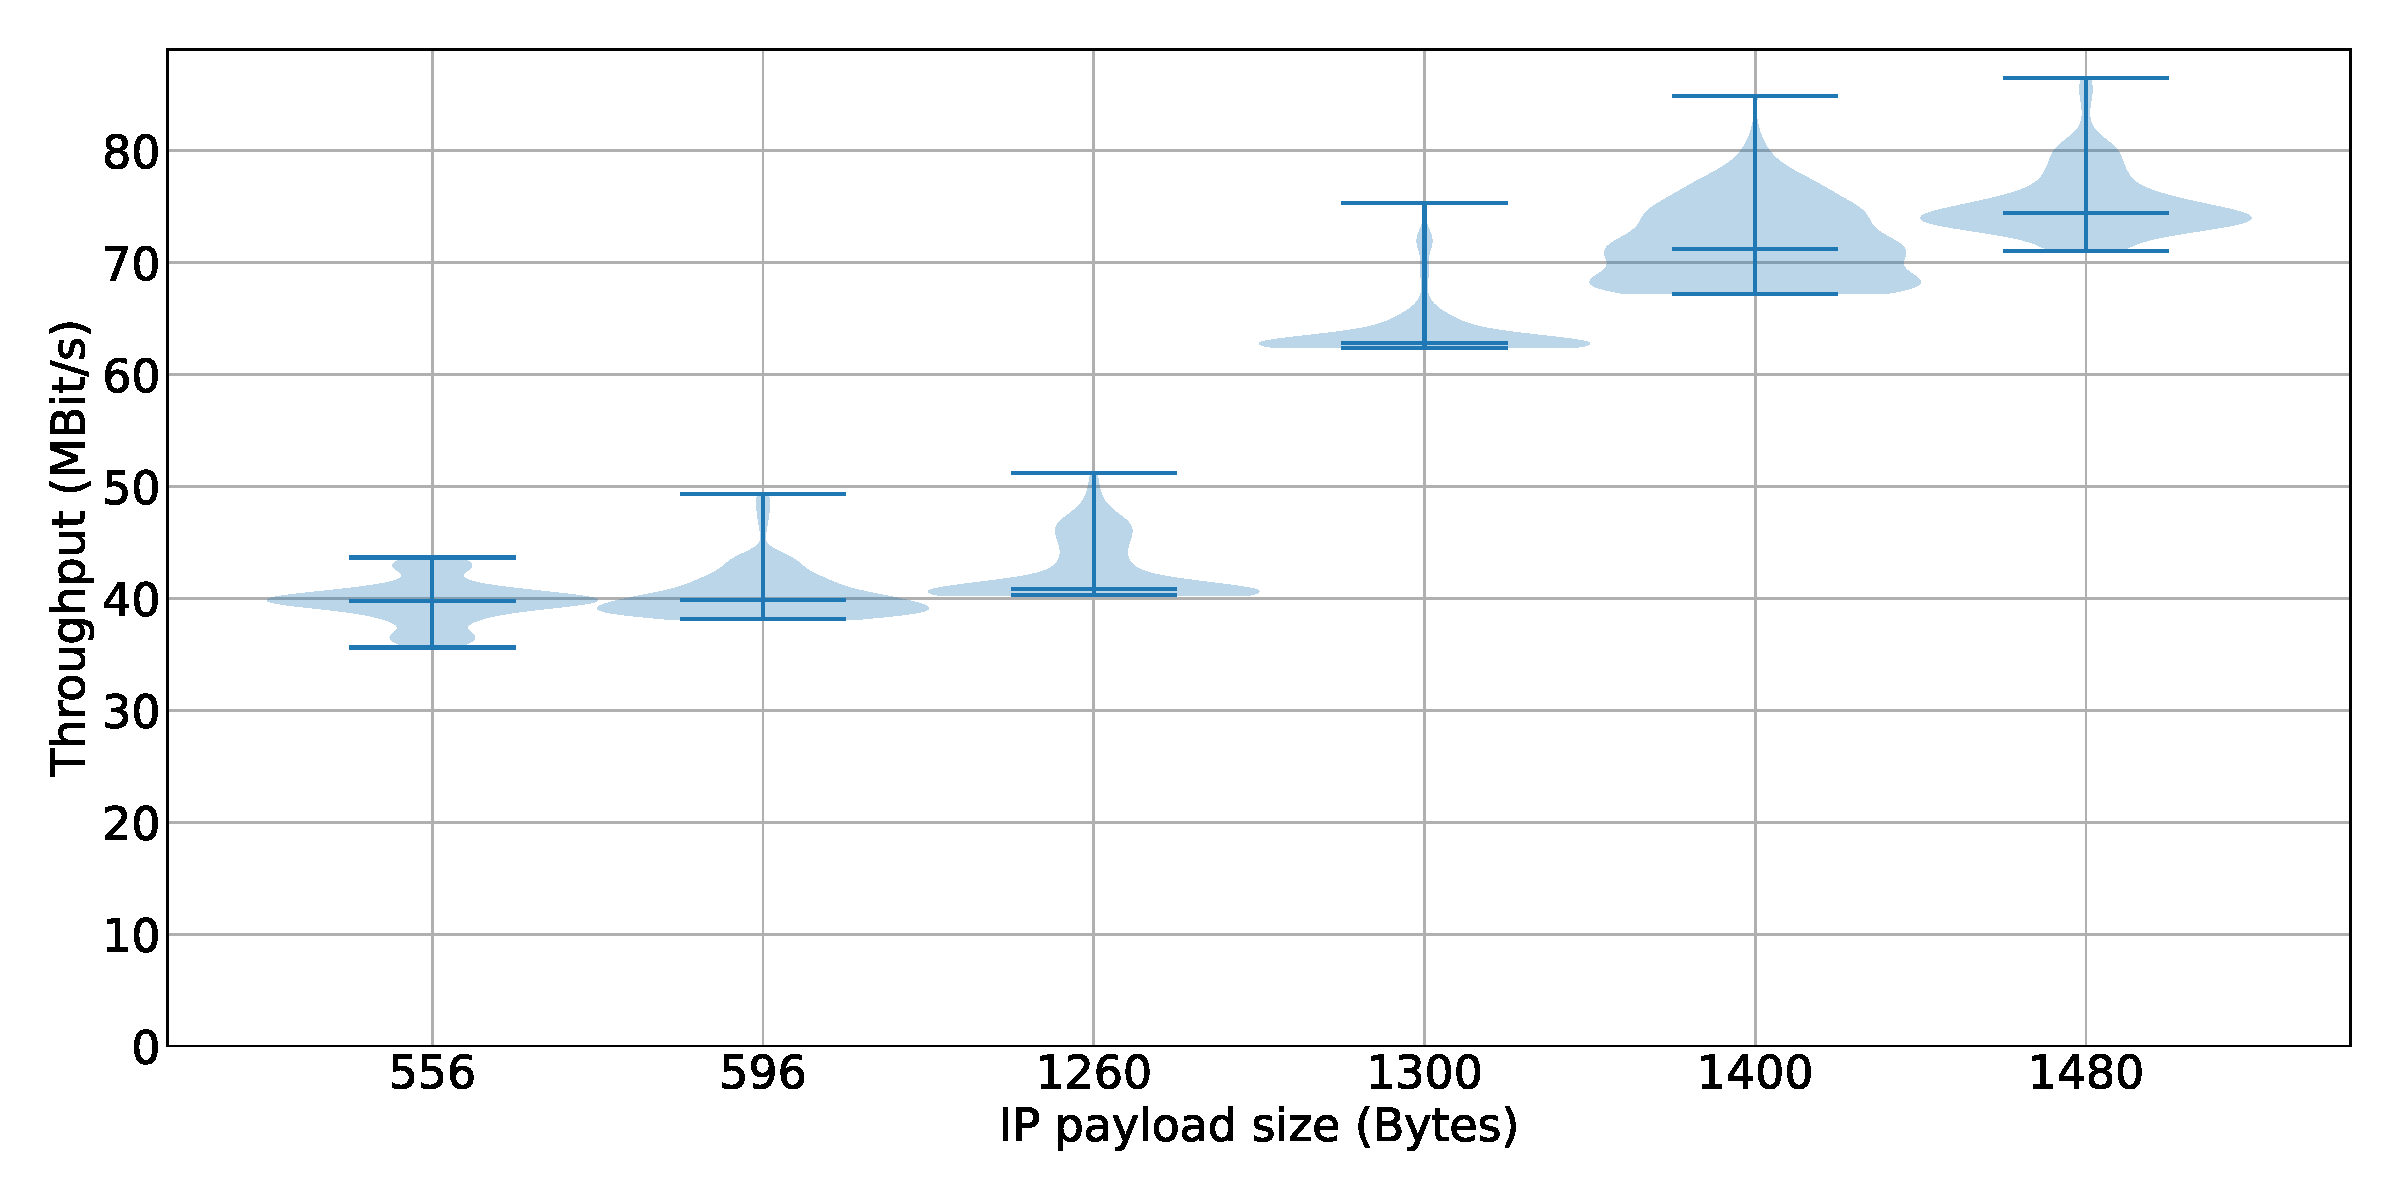
\includegraphics[draft=false,width=0.9\textwidth]{figures/Graphs/graph-1-mtu/throughput.pdf}
	\caption{Throughput for varying payload sizes}\label{fix:graph-1-mtu-throughput}
\end{figure}

The different measurements are always plotted on the x axis.

latency: violin plot: measurement, latency

packet duplicate: violin plot: measurement, ratio duplicate to total sent

packet dropped: violin plot: measurement, ratio dropped to total sent

throughput (with and without overhead): violin plot: measurement, throughput


move to chapter methodology:
one second buckets


We were unable to evaluate ICMPTX.
The program has a bug, where it crashes almost immediately after iperf3 starts sending data through the tunnel.
It fails with the error message \texttt{sendto: No buffer space available}.
The issue was mentioned previously \cite{icmptx-sendto-no-buffer-space-avaiable}.
The maintainer proposed two workarounds but using either one alone or both at the same time did not resolve the issue.
The problem seems to occur when trying to send data into the tunnel at a faster rate than the underlying link can support.
Tunnel software should be able to handle this case by dropping packets instead of crashing.


iodine

only one packet can be in flight, so usable throughput depends on latency and is generally very low

seems to not be true, since observed data rate was higher than expected

perhaps only the case in one direction?

Can not be measured reliably with our setup, would need improved setup, see figure



mostly see what we expected

we measure exactly the latency, loss and duplication we told the network emulator to simulate

measured throughput is influenced by number of dropped packets


Tor pluggable transports like obfs4 and Snowflake
meant for stream data like TCP, not UDP
\todo[inline]{Verify this claim more thouroughly!}

since we're only sending UDP packets, cannot be measured

would need a different test setup with a connection oriented data stream to test

instead of packet oriented

or some kind of UDP over TCP tunnel

this would also be influenced by congestion control algorithm

